\subsection{Inlet, Isolator, and Compression Duct [Thomas Satterly]}
\paragraph{Inlet}

The inlet was designed to provide the desired mass flow rate at cruise conditions whilst being capable of starting at Mach 5.5. Additionally, the geometry must be axisymmetric in order for a smooth flowpath from the inlet to the RDE. To satisfy these constraints, a simple conical inlet with variable geometry was selected. 
A cone with a half angle of 5 degrees was selected to minimize pressure loss and heat transfer at the inlet. By solving the Taylor-Maccoll equations for a conical shock, the outer cowl was sized to place the shock at the cowl during cruise conditions. In order to avoid mass flow loss and extra drag due to spillage at the starting conditions, a variable geometry cone is desirable to keep the shock at the cowl. This is achieved by shifting the inlet cone axially during acceleration. For this inlet to perform as desired between Mach 5.5 and 6.5, the cone only needs to be able to move 2.6 cm in total. The extremes of the cone position, as well as the shock placement on the cowl, can be seen in Figure \ref{fig:coneVari}.

\begin{figure}[H]
\begin{center}
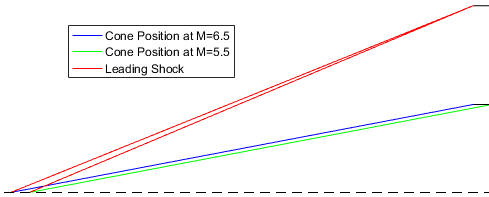
\includegraphics[width=0.6\textwidth]{coneVari}
\caption{$C_D$ v. Mach}
\label{fig:coneVari}
\end{center}
\end{figure}

\paragraph{Isolator}

    The isolator was designed using a combination of industry accepted assumptions and correlations rather than a complete shock train analysis, given that this is a preliminary design. A constant area annular duct was chosen for the general geometry, as it would transition easily from the conical inlet and minimally disrupt the flow as it approaches the combustor. 
A major assumption made was that the exit Mach from the isolator is 1/2 of the entrance Mach to the inlet. Typically, this ratio is closer to 1/3, but a great advantage of the RDE is the possibility to maintain combustion at high Mach numbers. If this design exercise is to be forward-looking, it is not unreasonable to assume that more capable isolators will also be developed in the future. 
    The total pressure ratio of the isolator is taken from MilStd 5007D \cite{milstd5007D}, which is a relationship between free stream Mach and total pressure ratio that has been standardized to allow for preliminary design and sizing of an inlet and isolator system without spending valuable resources on an extensive flow analysis. Finally, the length of the inlet was derived using the Waltrup and Billig correlations \cite{waltrup}.


\paragraph{Compression Duct}

    The final piece needed before reaching the combustor is a compression duct between the isolator and RDE entrance. The compression duct serves many purposes that ultimately balances the RDE operational properties with the upstream properties already set by the inlet and isolator system. The inlet sets the mass flow rate while the isolator sets the total pressure, total temperature, and Mach of the flow before reaching the compression duct. The RDE, on the other hand, was designed to operate at a specific static pressure, mass flow rate, and has a prescribed geometry. The compression duct unifies these components by delivering the flow from the inlet and isolator system, which have their own prescribed geometry, to the RDE such that flow properties are not violated. This was accomplished primarily by iterating on possible RDE operational conditions and geometry and verifying that, if the compression duct is isentropic, the upstream flow can be successfully delivered to the RDE within its design specifications. 
